\scanpage{18}
\margin{\figure{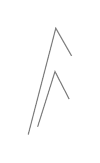
\begin{tikzpicture}[x=1cm,y=1cm]\draw[gray] (0,0)--(.35,1.35)--(.55,1.0);\draw[gray] (.12,.1)--(.34,.8)--(.52,.45);\end{tikzpicture}}}
\deleted{EGA IV $4^{\mathrm o}$ (2èmes épreuves).

P.164\unsure{n|m},note de bas de page, ajouter: ``La Si $f$ est supposé localement de présentation finie ou quasi-projectif, la référence à (18.12.13) peut d'ailleurs se remplacer par une référence à (8.12.8) resp. à (8.12.6).''

Page 165, ligne 9, manque virgule après $X_j$.

Page 166, deux lignes précédant 18.10.8? , les introduire par ``\uline{Remarque} 18.10.17.2.'' , ou (si la place manque), par le seul numéro de référence 18.10.17.2.

Page 187, c'est bien triste d'avoir une démonstration aussi peu parlante de la dernière assertion de (iii), qui est essentiellement triviale et devrait tenir en deux lignes, en \deleted{remarquant} \inserted{utilisant} simplement que si un idéal $\underline J$ est engendré par une suite $\underline O_X$-régulirère $(f_i)$, les $f_i\bmod\underline J^2$ forment une base de $\underline J/\underline J^2$ sur $\underline O_X/\underline J$; cela dit, on trouve évidemment pour le terme médian de (19.1.5.1) une base (localement) se décomposant en deux paquets, dont l'un et l'autre définissent resp. des bases du sous-module et du module quotient. Est-il encore possible de changer le texte en conséquence ?

Page 219, 19.7.5. (i) la référence à (11.3.4) est encore canulée, mettre (6.10.1) !

Page 224, ligne -8, \unsure{ya-t-il|y a-t-il} une référence pour le fait (effectivement vrai) qu'un module est limite inductive \inserted{filtrante} de modules de prés. finie ? Bien sur, on peut toujours s'en tirer en deux crans si on ne veut l'utiliser ($M$ est $\lim$ de ses sous-modules de type fini; un module de type fini est $\lim$ de modules de prés. finie).

Page 225, fin du par. 19, remplacer trois fois F par H (aux lignes -3 et -1 du paragraphe).}

Page 245, référence à $\mathrm{ERR}_{\mathrm{IV}}$ à compléter.
Page 271, ligne 9, manque point-et-virgule après formule.
\mspage{17}
